\section{作业整理}

\begin{remarkBox}{使用说明}
本章把第二章至第八章作业整理为便于期末复习的题目与解题流程。每道题保留核心条件、关键公式和最终结论；若原答案中存在明显计算问题，整理时按信息论公式重新核算。
\end{remarkBox}

作业题的价值不在于背答案，而在于训练三类能力：先把文字题翻译成概率模型，再选择熵、互信息、熵率、编码公式、判决准则或信道容量公式，最后检查结果是否符合基本性质。例如互信息不能为负，平均码长不能小于信源熵，马氏源熵率不能超过零阶熵，信道容量不能超过输出字母表最大熵。

\subsection{第二章作业：离散信息量、熵与互信息}

\begin{example}
\label{hw:ch2-bayes-information}
\textbf{贝叶斯公式与信息量}：某地区女孩中有 $25\%$ 是大学生，在女大学生中有 $75\%$ 身高 $1.6$ 米以上，而女孩中身高 $1.6$ 米以上者占总数的一半。若得知“身高 $1.6$ 米以上的某女孩是大学生”，求该消息的信息量。

\noindent \textbf{解题流程}：\\[2pt]
步骤一：先用贝叶斯公式求条件概率。\\
步骤二：再用自信息公式 $I(x)=-\log_2p(x)$。\\
步骤三：检查概率越小，信息量越大。

\textbf{解}：设 $A$ 表示“大学生”，$B$ 表示“身高不低于 $1.6$ 米”。由题意
\[
P(A)=0.25,
\qquad
P(B\mid A)=0.75,
\qquad
P(B)=0.5.
\]
由贝叶斯公式，
\[
P(A\mid B)=\frac{P(B\mid A)P(A)}{P(B)}
=\frac{0.75\times0.25}{0.5}=0.375=\frac38.
\]
因此该消息的信息量为
\[
I(A\mid B)=-\log_2\frac38
=\log_2\frac83
\approx1.415\text{ bit}.
\]
\end{example}

\begin{example}
\label{hw:ch2-entropy-conditional-mutual-information}
\textbf{熵、条件熵与互信息}：随机变量 $X,Y\in\{0,1\}$ 的联合概率为
\[
\begin{array}{c|cc}
 & Y=0 & Y=1\\
\hline
X=0 & \frac18 & \frac38\\
X=1 & \frac38 & \frac18
\end{array}
\]
令 $Z=XY$。求主要熵、条件熵和互信息。

\noindent \textbf{解题流程}：\\[2pt]
步骤一：先由联合表求边缘分布与 $Z$ 的分布。\\
步骤二：用联合熵和链式法则求条件熵。\\
步骤三：用 $I(X;Y)=H(X)+H(Y)-H(X,Y)$ 及条件互信息公式。

\textbf{解}：边缘分布为
\[
P(X=0)=P(X=1)=\frac12,
\qquad
P(Y=0)=P(Y=1)=\frac12,
\]
所以
\[
H(X)=H(Y)=1.
\]
由于 $Z=XY$，只有 $X=Y=1$ 时 $Z=1$，故
\[
P(Z=0)=\frac78,
\qquad
P(Z=1)=\frac18,
\]
从而
\[
H(Z)=H\left(\frac18\right)
=-\frac78\log_2\frac78-\frac18\log_2\frac18
\approx0.544\text{ bit}.
\]

联合熵
\[
H(X,Y)=-2\cdot\frac18\log_2\frac18-2\cdot\frac38\log_2\frac38
\approx1.811\text{ bit}.
\]
由于 $Z$ 由 $X,Y$ 确定，
\[
H(X,Y,Z)=H(X,Y)\approx1.811\text{ bit}.
\]
由 $(X,Z)$ 的分布
\[
P(0,0)=\frac12,
\quad P(1,0)=\frac38,
\quad P(1,1)=\frac18,
\]
可得
\[
H(X,Z)=H(Y,Z)\approx1.406\text{ bit}.
\]

于是
\[
H(X\mid Y)=H(Y\mid X)=H(X,Y)-1\approx0.811,
\]
\[
H(X\mid Z)=H(Y\mid Z)=H(X,Z)-H(Z)\approx0.862,
\]
\[
H(Z\mid X)=H(Z\mid Y)=H(X,Z)-H(X)\approx0.406.
\]
因为 $Z$ 由 $X,Y$ 确定，所以
\[
H(Z\mid X,Y)=0.
\]
又因为给定 $Y,Z$ 可唯一确定 $X$，给定 $X,Z$ 可唯一确定 $Y$，所以
\[
H(X\mid Y,Z)=0,
\qquad
H(Y\mid X,Z)=0.
\]

互信息为
\[
I(X;Y)=H(X)+H(Y)-H(X,Y)
\approx0.189\text{ bit},
\]
\[
I(X;Z)=H(X)+H(Z)-H(X,Z)
\approx0.138\text{ bit},
\]
\[
I(Y;Z)\approx0.138\text{ bit}.
\]
条件互信息例如
\[
I(Y;Z\mid X)=H(Y\mid X)-H(Y\mid X,Z)
\approx0.811\text{ bit}.
\]
\end{example}

\begin{example}
\label{hw:ch2-weather-mutual-information}
\textbf{天气预报准确率与平均互信息}：设 $X$ 表示实际天气，$Y$ 表示预报天气，取值均为“雨/无雨”。联合概率为
\[
P(\text{雨},\text{雨})=\frac18,
\quad
P(\text{雨},\text{无雨})=\frac1{16},
\]
\[
P(\text{无雨},\text{雨})=\frac3{16},
\quad
P(\text{无雨},\text{无雨})=\frac{10}{16}.
\]
求预报准确率和平均互信息，并与“总是预报无雨”比较。

\textbf{解}：准确率为
\[
P(X=Y)=\frac18+\frac{10}{16}=\frac{12}{16}=0.75.
\]
边缘分布为
\[
P_X=\left(\frac3{16},\frac{13}{16}\right),
\qquad
P_Y=\left(\frac5{16},\frac{11}{16}\right).
\]
计算得
\[
H(X)\approx0.6962,
\qquad
H(Y)\approx0.8960,
\qquad
H(X,Y)\approx1.5016.
\]
因此
\[
I(X;Y)=H(X)+H(Y)-H(X,Y)
\approx0.0906\text{ bit}.
\]
若总是预报“无雨”，准确率为
\[
P(X=\text{无雨})=\frac{13}{16}=0.8125,
\]
但预报变量为常量，故
\[
I(X;Y)=0.
\]
所以“总是无雨”的准确率更高，但从信息论角度看它不提供关于天气变化的信息；原预报准确率较低，却有正互信息，因而更有信息意义。
\end{example}

\begin{warningBox}{第二章作业易错点}
\begin{itemize}
  \item 自信息用事件真实发生后的概率计算，先用贝叶斯公式求后验概率，再取 $-\log_2$。
  \item 互信息一定非负；若算出负数，通常是联合熵或边缘熵算错。
  \item 准确率高不等于信息量大。始终输出同一个结果可能准确率不低，但互信息为 $0$。
\end{itemize}
\end{warningBox}

\subsection{第三章作业：离散信源与马氏源}

\begin{example}
\label{hw:ch3-homogeneous-markov-entropy}
\textbf{齐次马氏链熵计算}：设齐次马氏链 $X_1,X_2,\dots$ 取值于 $\{1,2,3\}$，转移概率矩阵为
\[
P=\begin{bmatrix}
1/2&1/4&1/4\\
2/3&0&1/3\\
2/3&1/3&0
\end{bmatrix},
\]
初始分布为
\[
P(X_1)=\left(\frac12,\frac14,\frac14\right).
\]
求 $H(X_1X_2X_3)$、平均符号熵和熵率。

\noindent \textbf{解题流程}：\\[2pt]
步骤一：用马氏链链式法则拆成 $H(X_1)+H(X_2\mid X_1)+H(X_3\mid X_2)$。\\
步骤二：每个条件熵是当前状态分布对“行熵”的加权平均。\\
步骤三：熵率使用平稳分布加权行熵。

\textbf{解}：初始熵为
\[
H(X_1)=H\left(\frac12,\frac14,\frac14\right)=1.5\text{ bit}.
\]
三行转移分布的熵分别为
\[
h_1=H\left(\frac12,\frac14,\frac14\right)=1.5,
\]
\[
h_2=h_3=H\left(\frac23,\frac13\right)\approx0.918.
\]
因此
\[
H(X_2\mid X_1)=\frac12h_1+\frac14h_2+\frac14h_3\approx1.209.
\]
下一时刻分布为
\[
P(X_2)=P(X_1)P=\left(\frac7{12},\frac5{24},\frac5{24}\right),
\]
故
\[
H(X_3\mid X_2)=\frac7{12}h_1+\frac5{24}h_2+\frac5{24}h_3
\approx1.2575.
\]
于是
\[
H(X_1X_2X_3)\approx1.5+1.209+1.2575=3.9665\text{ bit},
\]
\[
\frac13H(X_1X_2X_3)\approx1.322\text{ bit/符号}.
\]

平稳分布满足 $\pi P=\pi$，可得
\[
\pi=\left(\frac8{14},\frac3{14},\frac3{14}\right).
\]
所以熵率为
\[
H_\infty=\sum_i\pi_i h_i
=\frac8{14}\cdot1.5+\frac3{14}\cdot0.918+\frac3{14}\cdot0.918
\approx1.25\text{ bit/符号}.
\]
若零阶最大熵取
\[
H_0=\log_2 3\approx1.585,
\]
冗余度为
\[
\gamma=1-\frac{H_\infty}{H_0}
\approx21.1\%.
\]
\end{example}

\begin{example}
\label{hw:ch3-symmetric-first-order-markov-source}
\textbf{对称一阶马氏源}：信源符号集为 $\{0,1,2\}$。保持原状态的概率为 $1-p$，转移到另外两个状态的概率各为 $p/2$。求平稳分布、熵率、最大熵率对应的 $p$，并比较无记忆看法下的熵。

\textbf{解}：转移矩阵为
\[
P=\begin{bmatrix}
1-p&p/2&p/2\\
p/2&1-p&p/2\\
p/2&p/2&1-p
\end{bmatrix}.
\]

\begin{center}
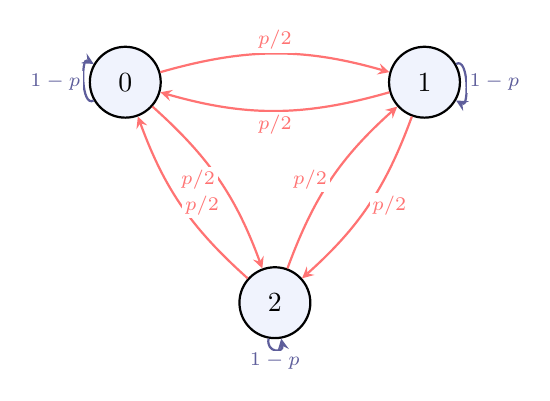
\begin{tikzpicture}[
    >=stealth,
    scale=1.0,
    state/.style={draw, circle, thick, minimum size=0.9cm, fill=RoyalBlue!8, font=\bfseries},
    edge label/.style={font=\scriptsize, fill=white, inner sep=1pt}
  ]
  \node[state] (s0) at (0,1.8) {$0$};
  \node[state] (s1) at (3.8,1.8) {$1$};
  \node[state] (s2) at (1.9,-1.0) {$2$};

  \draw[->, thick, MidnightBlue!70]
    (s0) .. controls +(-150:0.65) and +(-210:0.65) .. (s0)
    node[midway, left, edge label] {$1-p$};
  \draw[->, thick, MidnightBlue!70]
    (s1) .. controls +(30:0.65) and +(330:0.65) .. (s1)
    node[midway, right, edge label] {$1-p$};
  \draw[->, thick, MidnightBlue!70]
    (s2) .. controls +(-100:0.65) and +(-80:0.65) .. (s2)
    node[midway, below, edge label] {$1-p$};

  \draw[->, thick, red!55] (s0) to[bend left=16]
    node[edge label, above] {$p/2$} (s1);
  \draw[->, thick, red!55] (s1) to[bend left=16]
    node[edge label, below] {$p/2$} (s0);
  \draw[->, thick, red!55] (s0) to[bend left=14]
    node[edge label, left] {$p/2$} (s2);
  \draw[->, thick, red!55] (s2) to[bend left=14]
    node[edge label, right] {$p/2$} (s0);
  \draw[->, thick, red!55] (s1) to[bend left=14]
    node[edge label, right] {$p/2$} (s2);
  \draw[->, thick, red!55] (s2) to[bend left=14]
    node[edge label, left] {$p/2$} (s1);
\end{tikzpicture}
\end{center}

该矩阵为双随机矩阵，且状态完全对称，因此平稳分布为
\[
\pi_0=\pi_1=\pi_2=\frac13.
\]
每一行转移分布均为
\[
\left(1-p,\frac p2,\frac p2\right),
\]
所以熵率为
\[
H_\infty
=-(1-p)\log_2(1-p)-p\log_2\frac p2.
\]
当三项转移概率相等时熵最大：
\[
1-p=\frac p2,
\qquad
p=\frac23.
\]
此时
\[
H_\infty=\log_2 3.
\]
当 $p=0$ 时，状态不变，信源确定，
\[
H_\infty=0.
\]
当 $p=1$ 时，状态必定转移到另外两个状态之一，且二者等概，
\[
H_\infty=1\text{ bit/符号}.
\]
若忽略记忆性，仅按平稳分布看作无记忆信源，则
\[
H=H\left(\frac13,\frac13,\frac13\right)=\log_2 3.
\]
\end{example}

\subsection{第四章作业：连续信源与微分熵}

\begin{example}
\label{hw:ch4-independent-gaussian-linear-combination}
\textbf{独立高斯变量的线性组合}：设连续随机变量 $X,Y$ 的联合密度为
\[
p(x,y)=\frac{1}{2\pi\sigma_x\sigma_y}
\exp\left\{-\left[\frac{(x-m_x)^2}{2\sigma_x^2}+\frac{(y-m_y)^2}{2\sigma_y^2}\right]\right\}.
\]
令 $U=X+Y$、$V=X-Y$。求 $p(u)$、$p(v)$、$h(U)$、$h(V)$ 和 $I(U;V)$。

\textbf{解}：联合密度可分解为 $p(x)p(y)$，所以
\[
X\sim N(m_x,\sigma_x^2),
\qquad
Y\sim N(m_y,\sigma_y^2),
\]
且 $X,Y$ 独立。由高斯线性组合性质，
\[
U\sim N(m_x+m_y,\sigma_x^2+\sigma_y^2),
\]
\[
V\sim N(m_x-m_y,\sigma_x^2+\sigma_y^2).
\]
因此
\[
p(u)=\frac{1}{\sqrt{2\pi(\sigma_x^2+\sigma_y^2)}}
\exp\left\{-\frac{[u-(m_x+m_y)]^2}{2(\sigma_x^2+\sigma_y^2)}\right\},
\]
\[
p(v)=\frac{1}{\sqrt{2\pi(\sigma_x^2+\sigma_y^2)}}
\exp\left\{-\frac{[v-(m_x-m_y)]^2}{2(\sigma_x^2+\sigma_y^2)}\right\}.
\]
高斯微分熵为
\[
h(U)=h(V)=\frac12\ln\left[2\pi e(\sigma_x^2+\sigma_y^2)\right].
\]
线性变换
\[
\begin{bmatrix}U\\V\end{bmatrix}
=
\begin{bmatrix}1&1\\1&-1\end{bmatrix}
\begin{bmatrix}X\\Y\end{bmatrix}
\]
的行列式绝对值为 $2$，因此
\[
h(U,V)=h(X,Y)+\ln2.
\]
又
\[
h(X,Y)=\ln(2\pi e\sigma_x\sigma_y),
\]
所以
\[
I(U;V)=h(U)+h(V)-h(U,V)
=\ln\frac{\sigma_x^2+\sigma_y^2}{2\sigma_x\sigma_y}.
\]
\end{example}

\begin{example}
\label{hw:ch4-correlated-gaussian-linear-transform}
\textbf{相关高斯变量与二维线性变换}：设 $X,Y$ 均值为 $0$，方差分别为 $1,4$，相关系数为 $0.5$。令
\[
U=2X+Y,
\qquad
V=X-Y.
\]
求 $h(X)$、$h(Y)$、协方差矩阵 $K_Z$、$h(X,Y)$ 和 $h(U,V)$。

\textbf{解}：由高斯微分熵公式，
\[
h(X)=\frac12\ln(2\pi e),
\qquad
h(Y)=\frac12\ln(8\pi e).
\]
协方差为
\[
\Cov(X,Y)=\rho\sigma_X\sigma_Y=0.5\times1\times2=1,
\]
所以
\[
K_Z=\begin{bmatrix}1&1\\1&4\end{bmatrix}.
\]
其行列式为
\[
|K_Z|=3.
\]
二维高斯微分熵为
\[
h(X,Y)=\frac12\ln\left[(2\pi e)^2|K_Z|\right]
=\ln(2\pi e\sqrt3).
\]
线性变换矩阵为
\[
A=\begin{bmatrix}2&1\\1&-1\end{bmatrix},
\qquad
|\det A|=3.
\]
因此
\[
h(U,V)=h(X,Y)+\ln|\det A|
=\ln(6\pi e\sqrt3).
\]
\end{example}

\begin{formulaBox}{第四章作业常用公式}
一维高斯微分熵：
\[
h(X)=\frac12\ln(2\pi e\sigma^2).
\]
二维高斯微分熵：
\[
h(Z)=\frac12\ln\left[(2\pi e)^2|K_Z|\right].
\]
可逆线性变换 $Y=AX$ 满足
\[
h(Y)=h(X)+\ln|\det A|.
\]
\end{formulaBox}

\subsection{第五章作业：无失真信源编码}

\begin{example}
\label{hw:ch5-binary-source-fixed-length-coding}
\textbf{无记忆二元信源等长编码}：无记忆二元信源中，$P(0)=0.995$，$P(1)=0.005$。信源输出长度 $N=100$ 的二元序列，只对含有不超过 $3$ 个 $1$ 的序列一一编码。求二元等长码最小码长和错误概率。

\noindent \textbf{解题流程}：\\[2pt]
步骤一：统计需要编码的序列数。\\
步骤二：用 $2^l\ge M$ 求最小等长码长度。\\
步骤三：错误概率是未被编码的序列概率。

\textbf{解}：含有 $k$ 个 $1$ 的长度 $100$ 二元序列数为 $\binom{100}{k}$。需要编码的序列总数为
\[
M=\sum_{k=0}^{3}\binom{100}{k}
=166751.
\]
二元等长码码长 $l$ 满足
\[
2^l\ge M,
\]
所以
\[
l_{\min}=\left\lceil\log_2 166751\right\rceil=18.
\]
错误概率为序列中 $1$ 的个数大于 $3$ 的概率：
\[
P_e=1-\sum_{k=0}^{3}\binom{100}{k}(0.005)^k(0.995)^{100-k}
\approx0.001673.
\]
\end{example}

\begin{example}
\label{hw:ch5-huffman-coding}
\textbf{Huffman 编码}：离散无记忆信源有 $8$ 个符号，概率为
\[
\begin{array}{c|cccccccc}
\text{信源符号} & a_0&a_1&a_2&a_3&a_4&a_5&a_6&a_7\\
\hline
\text{概率} & 0.1&0.1&0.1&0.1&0.1&0.4&0.05&0.05
\end{array}
\]
求一组二元 Huffman 码、平均码长、码长方差、信源熵和编码效率。

\textbf{解}：为使码长方差较小，等概率节点合并时尽量平衡码长。可得到码长分布
\[
l_0=l_1=l_2=l_3=l_4=3,
\qquad
l_5=2,
\qquad
l_6=l_7=4.
\]
一组满足该码长分布的 Huffman 码为
\[
\begin{array}{c|cccccccc}
\text{信源符号} & a_0&a_1&a_2&a_3&a_4&a_5&a_6&a_7\\
\hline
\text{码字} & 001&010&011&100&101&11&0000&0001
\end{array}
\]
它满足 Kraft 等式
\[
5\cdot2^{-3}+2^{-2}+2\cdot2^{-4}=1.
\]
平均码长为
\[
\bar L=5\times0.1\times3+0.4\times2+2\times0.05\times4=2.7.
\]
码长方差为
\[
\sigma_L^2=\sum_i p_i(l_i-\bar L)^2
\]
\[
=5\times0.1(3-2.7)^2+0.4(2-2.7)^2+2\times0.05(4-2.7)^2
=0.41.
\]
信源熵为
\[
H(X)=-5\times0.1\log_2 0.1-0.4\log_2 0.4-2\times0.05\log_2 0.05
\approx2.6219\text{ bit/符号}.
\]
编码速率取平均码长
\[
R=\bar L=2.7\text{ bit/符号},
\]
编码效率为
\[
\eta=\frac{H(X)}{\bar L}\approx\frac{2.6219}{2.7}=0.9711.
\]
\end{example}

\subsection{第六章作业：离散信道及其容量}

\begin{example}
\label{hw:ch6-3-channel-capacity}
\textbf{2 输入 3 输出信道容量（6.3）}：一信道的转移概率矩阵为
\[
P=
\begin{pmatrix}
\frac{2}{3} & \frac{1}{3} & 0\\
0 & \frac{1}{3} & \frac{2}{3}
\end{pmatrix}.
\]
求：(1) 该信道达到容量时的输出概率分布；(2) 该信道容量。

\noindent \textbf{解题流程}：\\[2pt]
步骤一：设输入分布 $P(X=0)=p$，写出输出分布。\\
步骤二：观察两行条件熵相同，把最大化 $I(X;Y)$ 化为最大化 $H(Y)$。\\
步骤三：利用熵的凹性，使可变的输出概率尽量均匀。

\textbf{解}：设
\[
P(X=0)=p,
\qquad
P(X=1)=1-p.
\]
则输出分布为
\[
P_Y=\left(\frac{2p}{3},\frac13,\frac{2(1-p)}{3}\right).
\]
两行转移概率的熵相同，因此
\[
H(Y\mid X)=H\left(\frac23,\frac13,0\right)=h_2\left(\frac13\right),
\]
其中
\[
h_2(q)=-q\log_2q-(1-q)\log_2(1-q).
\]
于是
\[
I(X;Y)=H(Y)-h_2\left(\frac13\right).
\]

因为 $P(Y=1)=1/3$ 固定，剩余概率 $2/3$ 在 $Y=0$ 与 $Y=2$ 上分配。由熵的凹性，$H(Y)$ 在
\[
P(Y=0)=P(Y=2)=\frac13
\]
时最大，此时 $p=1/2$。所以达到容量时的输出分布为
\[
P_Y^*=\left(\frac13,\frac13,\frac13\right).
\]
信道容量为
\[
C=\log_2 3-h_2\left(\frac13\right)
\]
\[
=\log_2 3+\frac13\log_2\frac13+\frac23\log_2\frac23
=\frac23\text{ bit/符号}.
\]
\end{example}

\begin{example}
\label{hw:ch6-14-cascaded-bsc-erasure-capacity}
\textbf{BSC 与删除型信道级联容量（6.14）}：给定级联信道
\[
X\to Y\to Z,
\]
其中 $X,Y\in\{0,1\}$，$Z\in\{0,1,2\}$。$X$ 到 $Y$ 为交叉概率为 $\varepsilon$ 的二元对称信道：
\[
P_{Y\mid X}=
\begin{pmatrix}
1-\varepsilon & \varepsilon\\
\varepsilon & 1-\varepsilon
\end{pmatrix}.
\]
$Y$ 到 $Z$ 的转移概率为
\[
P_{Z\mid Y=0}=\left(\frac34,0,\frac14\right),
\qquad
P_{Z\mid Y=1}=\left(0,\frac34,\frac14\right).
\]

\begin{center}
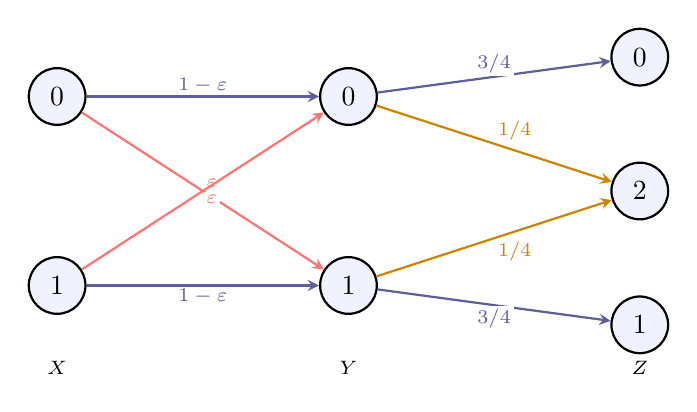
\begin{tikzpicture}[
    >=stealth,
    scale=1.0,
    node/.style={draw, circle, thick, minimum size=0.72cm, fill=RoyalBlue!8},
    edge label/.style={font=\scriptsize, fill=white, inner sep=1pt}
  ]
  \node[node] (x0) at (0,1.2) {$0$};
  \node[node] (x1) at (0,-1.2) {$1$};
  \node[node] (y0) at (3.7,1.2) {$0$};
  \node[node] (y1) at (3.7,-1.2) {$1$};
  \node[node] (z0) at (7.4,1.7) {$0$};
  \node[node] (z2) at (7.4,0) {$2$};
  \node[node] (z1) at (7.4,-1.7) {$1$};

  \draw[->, thick, MidnightBlue!70] (x0) -- node[edge label, above] {$1-\varepsilon$} (y0);
  \draw[->, thick, MidnightBlue!70] (x1) -- node[edge label, below] {$1-\varepsilon$} (y1);
  \draw[->, thick, red!55] (x0) -- node[edge label, above right] {$\varepsilon$} (y1);
  \draw[->, thick, red!55] (x1) -- node[edge label, below right] {$\varepsilon$} (y0);

  \draw[->, thick, MidnightBlue!70] (y0) -- node[edge label, above] {$3/4$} (z0);
  \draw[->, thick, MidnightBlue!70] (y1) -- node[edge label, below] {$3/4$} (z1);
  \draw[->, thick, Orange!80!black] (y0) -- node[edge label, above right] {$1/4$} (z2);
  \draw[->, thick, Orange!80!black] (y1) -- node[edge label, below right] {$1/4$} (z2);

  \node[font=\scriptsize] at (0,-2.25) {$X$};
  \node[font=\scriptsize] at (3.7,-2.25) {$Y$};
  \node[font=\scriptsize] at (7.4,-2.25) {$Z$};
\end{tikzpicture}
\end{center}

求 $X$ 与 $Y$、$Y$ 与 $Z$、$X$ 与 $Z$ 之间的信道容量，并求 $X\to Z$ 达到容量时的输入分布。

\noindent \textbf{解题流程}：\\[2pt]
步骤一：分别识别 $X\to Y$ 为 BSC，$Y\to Z$ 为删除概率 $1/4$ 的二元删除型信道。\\
步骤二：用矩阵相乘写出级联信道 $X\to Z$。\\
步骤三：利用对称性求最优输入分布，并单独检查 $\varepsilon=1/2$ 的退化情形。

\textbf{解}：二元熵函数记为
\[
h_2(q)=-q\log_2q-(1-q)\log_2(1-q).
\]

(1) $X\to Y$ 是交叉概率为 $\varepsilon$ 的 BSC，因此
\[
C_1=1-h_2(\varepsilon),
\]
当 $P(X=0)=P(X=1)=1/2$ 时达到容量。

(2) $Y\to Z$ 可看作删除概率为 $1/4$ 的二元删除型信道：以概率 $3/4$ 正确输出输入符号，以概率 $1/4$ 输出删除符号 $2$。所以
\[
C_2=\frac34\text{ bit/符号},
\]
当 $P(Y=0)=P(Y=1)=1/2$ 时达到容量。

(3) 级联后 $X\to Z$ 的转移概率为
\[
P_{Z\mid X=0}=\left(\frac{3(1-\varepsilon)}{4},\frac{3\varepsilon}{4},\frac14\right),
\]
\[
P_{Z\mid X=1}=\left(\frac{3\varepsilon}{4},\frac{3(1-\varepsilon)}{4},\frac14\right).
\]
设 $P(X=0)=p$，则
\[
P(Y=0)=p(1-\varepsilon)+(1-p)\varepsilon
=\varepsilon+p(1-2\varepsilon).
\]
由于
\[
P(Z=2)=\frac14
\]
恒定，要使 $H(Z)$ 最大，只需令
\[
P(Z=0)=P(Z=1)=\frac38,
\]
等价于
\[
P(Y=0)=P(Y=1)=\frac12.
\]
当 $\varepsilon\ne1/2$ 时，由
\[
\varepsilon+p(1-2\varepsilon)=\frac12
\]
得
\[
P(X=0)=P(X=1)=\frac12.
\]
此时输出分布为
\[
P_Z^*=\left(\frac38,\frac38,\frac14\right).
\]

条件熵为
\[
H(Z\mid X)=h_2\left(\frac14\right)+\frac34h_2(\varepsilon),
\]
而
\[
H(Z)=h_2\left(\frac14\right)+\frac34.
\]
因此
\[
C_3=H(Z)-H(Z\mid X)
=\frac34\left[1-h_2(\varepsilon)\right]\text{ bit/符号}.
\]
当 $\varepsilon=1/2$ 时，$X$ 与 $Z$ 独立，$C_3=0$，任意输入分布均可达到容量。
\end{example}

\subsection{第七章作业：有噪信道编码}

\begin{example}
\label{hw:ch7-2-fixed-code-length-transmission-rate}
\textbf{固定码长下的信息平均传输速率（7.2）}：信源消息为 $A,B,C,D$，编码为
\[
A\to00,
\quad B\to01,
\quad C\to10,
\quad D\to11.
\]
每个二进码元宽度为 $5\text{ms}$。求等概和非等概两种情况下的信息平均传输速率，其中非等概分布为
\[
P(A)=\frac15,
\quad P(B)=\frac14,
\quad P(C)=\frac14,
\quad P(D)=\frac3{10}.
\]

\noindent \textbf{解题流程}：\\[2pt]
步骤一：先由码元宽度求每个消息传输时间。\\
步骤二：计算信源熵 $H(X)$。\\
步骤三：用 $R=H(X)/T$ 求 bit/s。

\textbf{解}：每个消息编码为 $2$ 个二进码元，因此传输时间为
\[
T=2\times5\text{ms}=10\text{ms}=0.01\text{s}.
\]
信息平均传输速率为
\[
R=\frac{H(X)}{T}.
\]
等概时，
\[
H(X)=\log_2 4=2\text{ bit/消息},
\]
所以
\[
R=\frac{2}{0.01}=200\text{ bit/s}.
\]
非等概时，
\[
H(X)=-\frac15\log_2\frac15-\frac14\log_2\frac14
-\frac14\log_2\frac14-\frac3{10}\log_2\frac3{10}
\approx1.9855\text{ bit/消息}.
\]
因此
\[
R\approx\frac{1.9855}{0.01}=198.55\text{ bit/s}.
\]
\end{example}

\begin{example}
\label{hw:ch7-4-bsc-map-ml-decision}
\textbf{BSC 中 MAP 与 ML 判决（7.4）}：二元对称信道转移矩阵为
\[
P=
\begin{pmatrix}
1-p&p\\
p&1-p
\end{pmatrix},
\qquad p<\frac12.
\]
输入符号 $0,1$ 的概率分别为 $\omega,1-\omega$。求 MAP、ML 判决函数及平均错误率，并说明两准则何时相同。

\noindent \textbf{解题流程}：\\[2pt]
步骤一：MAP 对每个输出比较先验概率乘转移概率。\\
步骤二：ML 只比较转移概率。\\
步骤三：把 MAP 判决退化为“收到什么判什么”的条件与 ML 比较。

\textbf{解}：由于 $p<1/2$，有 $1-p>p$。MAP 准则为
\[
\hat x(y)=\arg\max_x P(X=x)P(Y=y\mid X=x).
\]
当 $Y=0$ 时比较 $\omega(1-p)$ 与 $(1-\omega)p$；当 $Y=1$ 时比较 $\omega p$ 与 $(1-\omega)(1-p)$。因此
\[
\hat x_{\mathrm{MAP}}(0)=
\begin{cases}
0,&\omega\ge p,\\
1,&\omega<p,
\end{cases}
\]
\[
\hat x_{\mathrm{MAP}}(1)=
\begin{cases}
0,&\omega\ge1-p,\\
1,&\omega<1-p.
\end{cases}
\]
平均正确概率为
\[
P_c=\max\{\omega(1-p),(1-\omega)p\}
+\max\{\omega p,(1-\omega)(1-p)\},
\]
所以
\[
P_{e,\mathrm{MAP}}=1-P_c.
\]
等价分段形式为
\[
P_{e,\mathrm{MAP}}=
\begin{cases}
\omega,&0\le\omega<p,\\
p,&p\le\omega<1-p,\\
1-\omega,&1-p\le\omega\le1.
\end{cases}
\]

ML 只比较转移概率。由于 $1-p>p$，收到什么就判为什么：
\[
\hat x_{\mathrm{ML}}(0)=0,
\qquad
\hat x_{\mathrm{ML}}(1)=1.
\]
平均错误率为
\[
P_{e,\mathrm{ML}}=\omega p+(1-\omega)p=p.
\]
两准则判决结果相同，当且仅当 MAP 也收到 $0$ 判 $0$、收到 $1$ 判 $1$，即
\[
p\le\omega<1-p.
\]
若等号处并列最大时允许按 ML 方式择优，可写为 $p\le\omega\le1-p$。
\end{example}

\begin{example}
\label{hw:ch7-14-nonuniform-map-reliability}
\textbf{非等概码字的 MAP 译码与可靠性比较（7.14）}：二元码长为 $4$ 的码字为
\[
W_1=0000,
\quad W_2=0011,
\quad W_3=1100,
\quad W_4=1111.
\]
码字通过单符号错误概率为 $p$ 的 BSC，且 $p<0.01$。码字概率为
\[
p(W_1)=\frac12,
\quad p(W_2)=p(W_3)=\frac18,
\quad p(W_4)=\frac14.
\]
求编码功率、最小平均差错率译码原则与错误率，并与不编码直接传输两个比特的系统比较。

\noindent \textbf{解题流程}：\\[2pt]
步骤一：编码功率按平均码字重量计算。\\
步骤二：最小平均差错率采用 MAP 译码。\\
步骤三：分别算编码和未编码系统的平均正确概率，再比较错误率量级。

\textbf{解}：码字重量为
\[
w(0000)=0,
\quad w(0011)=2,
\quad w(1100)=2,
\quad w(1111)=4.
\]
平均码字重量为
\[
\bar w=\sum_i p(W_i)w(W_i)
=\frac12\cdot0+\frac18\cdot2+\frac18\cdot2+\frac14\cdot4=\frac32.
\]
若按每码元平均功率计，则为
\[
\frac{\bar w}{4}=\frac38.
\]

使平均差错率最小的译码原则是 MAP：对接收字 $y$ 判为使 $p(W_i)P(y\mid W_i)$ 最大的码字。对 $p<0.01$，一组最优译码区域为
\[
D_1=\{0000,0001,0010,0100,0101,0110,1000,1001,1010\},
\]
\[
D_2=\{0011\},
\qquad
D_3=\{1100\},
\]
\[
D_4=\{0111,1011,1101,1110,1111\}.
\]
平均正确概率为
\[
P_c=\frac12\bigl[(1-p)^4+4p(1-p)^3+4p^2(1-p)^2\bigr]
\]
\[
+\frac18(1-p)^4+\frac18(1-p)^4
+\frac14\bigl[(1-p)^4+4p(1-p)^3\bigr].
\]
化简得
\[
P_c=1-p-p^2+p^3,
\]
故最小平均差错率为
\[
\bar p_E=1-P_c=p+p^2-p^3.
\]

若不采用编码，直接用 $2$ 位二进代码表示四个符号，并按 MAP 译码。取自然对应
\[
A\to00,
\quad B\to01,
\quad C\to10,
\quad D\to11.
\]
当 $p<0.01$ 时，最优判决区域为
\[
D_A=\{00,01,10\},
\qquad
D_D=\{11\}.
\]
平均正确概率为
\[
P_c'=\frac12\bigl[(1-p)^2+2p(1-p)\bigr]+\frac14(1-p)^2
=\frac34-\frac12p-\frac14p^2.
\]
因此未编码错误率为
\[
p_E'=1-P_c'=\frac14+\frac12p+\frac14p^2.
\]
由于 $p<0.01$，编码系统错误率约为 $p$，未编码系统错误率至少约为 $1/4$，编码显著提高可靠性。
\end{example}

\subsection{第八章作业：波形信道与高斯信道容量}

\begin{example}
\label{hw:ch8-3-amplitude-limited-uniform-noise-capacity}
\textbf{限幅加性均匀噪声信道容量（8.3）}：离散时间无记忆加性噪声信道满足
\[
Y=X+Z,
\]
输入 $X\in[-2,2]$，噪声 $Z$ 独立于 $X$，且在 $(-1,1)$ 上均匀分布。求 $I(X;Y)$、信道容量及达到容量时的输入输出分布。

\noindent \textbf{解题流程}：\\[2pt]
步骤一：利用加性独立噪声写 $I(X;Y)=h(Y)-h(Z)$。\\
步骤二：由输出支撑区间最大化差熵。\\
步骤三：构造离散输入，使平移后的噪声区间拼成均匀输出。

\textbf{解}：由于 $Y=X+Z$ 且 $X,Z$ 独立，
\[
I(X;Y)=h(Y)-h(Y\mid X)=h(Y)-h(Z).
\]
由
\[
X\in[-2,2],
\qquad
Z\in(-1,1),
\]
可知
\[
Y\in[-3,3].
\]
给定长度为 $6$ 的支撑区间时，差熵由均匀分布达到最大：
\[
h(Y)\le\log 6.
\]
又 $Z$ 在长度为 $2$ 的区间上均匀分布，
\[
h(Z)=\log 2.
\]
故信道容量为
\[
C=\log 6-\log 2=\log 3.
\]
若以 bit 为单位，则
\[
C=\log_2 3\text{ bit/符号}.
\]
达到容量时，输出应在 $[-3,3]$ 上均匀分布：
\[
f_Y(y)=\frac16,
\qquad -3<y<3.
\]
一种达到容量的输入分布为
\[
P\{X=-2\}=P\{X=0\}=P\{X=2\}=\frac13.
\]
此时三个噪声平移区间 $(-3,-1)$、$(-1,1)$、$(1,3)$ 拼成 $[-3,3]$ 上的均匀输出。
\end{example}

\begin{example}
\label{hw:ch8-10-parallel-gaussian-water-filling}
\textbf{四路并联高斯信道注水分配（8.10）}：四个并联高斯子信道的噪声方差为
\[
1,
\quad2,
\quad4,
\quad8.
\]
总输入能量限制为 $E$。分别求 $E=6$ 和 $E=18$ 时的最佳能量分配和每自由度容量。

\noindent \textbf{解题流程}：\\[2pt]
步骤一：设水位为 $\lambda$，能量分配为 $E_i=(\lambda-N_i)^+$。\\
步骤二：先假设激活若干低噪声子信道，算水位并检查是否超过下一噪声方差。\\
步骤三：代入 $C=\frac12\sum\log_2(\lambda/N_i)$。

\textbf{解}：注水分配满足
\[
E_i=(\lambda-N_i)^+,
\qquad
N_i=1,2,4,8,
\qquad
\sum_iE_i=E.
\]
每自由度容量为
\[
C=\frac12\sum_{i:E_i>0}\log_2\left(1+\frac{E_i}{N_i}\right)
=\frac12\sum_{i:E_i>0}\log_2\frac{\lambda}{N_i}.
\]

当 $E=6$ 时，若激活前三个子信道，
\[
\lambda=\frac{E+1+2+4}{3}=\frac{13}{3}<8,
\]
所以第 $4$ 个子信道不分配能量。最佳能量分配为
\[
(E_1,E_2,E_3,E_4)=\left(\frac{10}{3},\frac{7}{3},\frac{1}{3},0\right).
\]
容量为
\[
C=\frac12\log_2\left(\frac{13}{3}\cdot\frac{13}{6}\cdot\frac{13}{12}\right)
\approx1.673\text{ bit/自由度}.
\]

当 $E=18$ 时，四个子信道均被激活，
\[
\lambda=\frac{E+1+2+4+8}{4}=\frac{33}{4}>8.
\]
最佳能量分配为
\[
(E_1,E_2,E_3,E_4)=\left(\frac{29}{4},\frac{25}{4},\frac{17}{4},\frac14\right).
\]
容量为
\[
C=\frac12\log_2\left(\frac{33}{4}\cdot\frac{33}{8}\cdot\frac{33}{16}\cdot\frac{33}{32}\right)
\approx3.089\text{ bit/自由度}.
\]
\end{example}

\begin{example}
\label{hw:ch8-16-awgn-waveform-capacity}
\textbf{AWGN 波形信道容量计算（8.16）}：求下列加性高斯白噪声波形信道容量：电话线路信道带宽 $300\text{ Hz}$ 到 $3400\text{ Hz}$、信噪比 $30\text{ dB}$；深空通信信道带宽不受限，$P/N_0=10^6\text{ Hz}$；卫星通信信道带宽 $36\text{ MHz}$，$P/N_0=5\times10^8\text{ Hz}$。

\noindent \textbf{解题流程}：\\[2pt]
步骤一：带宽受限时用 Shannon 公式 $C=W\log_2(1+P/(N_0W))$。\\
步骤二：带宽不受限时取极限 $C=(P/N_0)\log_2 e$。\\
步骤三：注意 dB 与 Hz、MHz 的单位换算。

\textbf{解}：带宽受限 AWGN 信道容量为
\[
C=W\log_2\left(1+\frac{P}{N_0W}\right).
\]
带宽不受限时，容量极限为
\[
C=\frac{P}{N_0}\log_2 e.
\]

(1) 电话线路带宽为
\[
W=3400-300=3100\text{ Hz}.
\]
信噪比 $30\text{ dB}$ 对应
\[
\frac{S}{N}=10^{30/10}=1000.
\]
因此
\[
C=3100\log_2(1+1000)
\approx3.09\times10^4\text{ bit/s}.
\]

(2) 深空通信信道带宽不受限，且
\[
\frac{P}{N_0}=10^6\text{ Hz}.
\]
所以
\[
C=10^6\log_2e
\approx1.443\times10^6\text{ bit/s}.
\]

(3) 卫星通信信道带宽为
\[
W=36\text{ MHz}=36\times10^6\text{ Hz},
\]
且
\[
\frac{P}{N_0}=5\times10^8\text{ Hz}.
\]
故
\[
C=36\times10^6\log_2\left(1+\frac{5\times10^8}{36\times10^6}\right)
\approx1.403\times10^8\text{ bit/s}.
\]
\end{example}

\begin{warningBox}{作业综合易错点}
\begin{itemize}
  \item 马氏源熵率要用平稳分布加权各状态转移熵，不能直接把平稳分布的熵当熵率。
  \item 连续随机变量线性变换时，联合微分熵要加 $\ln|\det A|$，一维边缘熵不能直接相加来代替联合熵，除非独立。
  \item Huffman 编码平均码长应满足 $H(X)\le\bar L< H(X)+1$，效率不能超过 $1$。
  \item 等长码错误概率是未编码集合的总概率，不是未编码序列数除以全部序列数。
  \item 信道容量题不能默认输入等概；应先看信道是否对称，或通过最大化输出熵判断最优输入分布。
  \item 级联信道容量一般不能简单相乘；本章作业中出现 $C_3=\frac34[1-h_2(\varepsilon)]$ 是由具体 BSC 与删除型结构共同决定的。
  \item 当 $\varepsilon=1/2$ 时，BSC 输出与输入独立，级联后的 $X\to Z$ 容量退化为 $0$，需要单独说明。
  \item MAP 判决比较的是“先验概率 $\times$ 转移概率”，ML 只比较转移概率；输入不等概时二者可能不同。
  \item 注水分配算出负能量时，必须删去该子信道后重算水位，不能把负能量代入容量公式。
  \item 波形信道容量要区分 bit/自由度 与 bit/s；带宽受限和带宽不受限使用的公式不同。
\end{itemize}
\end{warningBox}

\subsection{公式速查表}

{\scriptsize
\noindent\begin{tabularx}{\textwidth}{@{}l>{\raggedright\arraybackslash}X@{}}
\toprule
\textbf{题型} & \textbf{关键公式 / 结论} \\
\midrule
自信息 & $I(x)=-\log_2p(x)$；条件信息量先求后验概率 \\
\midrule
互信息 & \textcolor{Red}{$I(X;Y)=H(X)+H(Y)-H(X,Y)\ge0$} \\
\midrule
马氏链联合熵 & $H(X_1^N)=H(X_1)+\sum_{i=2}^{N}H(X_i\mid X_{i-1})$ \\
\midrule
马氏源熵率 & \textcolor{Red}{$H_\infty=\sum_i\pi_iH(P_{i\cdot})$}，$\pi P=\pi$ \\
\midrule
高斯微分熵 & \textcolor{Red}{$h(X)=\frac12\ln(2\pi e\sigma^2)$} \\
\midrule
多元高斯熵 & $h(Z)=\frac12\ln[(2\pi e)^n|K_Z|]$ \\
\midrule
线性变换 & \textcolor{Red}{$h(AX)=h(X)+\ln|\det A|$}，要求 $A$ 可逆 \\
\midrule
等长编码长度 & \textcolor{Red}{$l_{\min}=\lceil\log_2M\rceil$} \\
\midrule
Huffman 平均码长 & $\bar L=\sum_i p_il_i$，码长方差 $\sigma_L^2=\sum_i p_i(l_i-\bar L)^2$ \\
\midrule
编码效率 & \textcolor{Red}{$\eta=H(X)/\bar L$} \\
\midrule
信道容量 & \textcolor{Red}{$C=\max_{p(x)}I(X;Y)$}，常转化为最大化 $H(Y)-H(Y\mid X)$ \\
\midrule
二元熵函数 & $h_2(q)=-q\log_2q-(1-q)\log_2(1-q)$ \\
\midrule
BSC 容量 & \textcolor{Red}{$C=1-h_2(\varepsilon)$}，等概输入达到容量 \\
\midrule
二元删除型信道 & 删除概率为 $\delta$ 时 $C=1-\delta$；第六章作业中 $\delta=1/4$ \\
\midrule
级联信道 & 先算整体转移矩阵 $P_{Z\mid X}=P_{Y\mid X}P_{Z\mid Y}$，再求 $\max I(X;Z)$ \\
\midrule
MAP 判决 & \textcolor{Red}{$\hat x(y)=\arg\max_x p(x)p(y\mid x)$}，可最小化平均错误率 \\
\midrule
ML 判决 & $\hat x(y)=\arg\max_x p(y\mid x)$；输入等概时与 MAP 等价 \\
\midrule
加性噪声信道 & 独立加性噪声下 $I(X;Y)=h(Y)-h(Z)$ \\
\midrule
注水分配 & $E_i=(\lambda-N_i)^+$，只对 $E_i>0$ 的子信道计入容量 \\
\midrule
AWGN 波形容量 & \textcolor{Red}{$C=W\log_2\left(1+\frac{P}{N_0W}\right)$}；无限带宽极限 $C=\frac{P}{N_0}\log_2e$ \\
\bottomrule
\end{tabularx}
}
